\section{GIRAF}
\begin{frame}
	\frametitle{GIRAF Project}
\end{frame}

\subsection{GIRAF Overview}

\begin{frame}
  \begin{center}
	\frametitle{Multiproject}
  \end{center}
\end{frame}

\begin{frame}
	\begin{center}
		\frametitle{Goals for the semester}
		\begin{itemize}
			\item \textit{A product that actually works and can be used} - 10/02-15
			\item Build upon existing features
			\item Quality over quantity
		\end{itemize}
	\end{center}
\end{frame}

\begin{frame}
	\frametitle{Roles and responsibility}
	\begin{columns}[T] % align columns
		\begin{column}{.48\textwidth}
			\begin{itemize}
				\item Redmine Wiki, Forum, general
				\item Server
				\item Webadmin
				\item Graphics/Fonts/etc
				\item Customer Representatives
				\item Git Handling
			\end{itemize}
		\end{column}%
		\hfill%
		\begin{column}{.48\textwidth}
			\begin{itemize}
				\item 
				\item code style
				\item Jenkins
				\item Scrum Process
				\item \textbf{Google Play}
				\item \textbf{Google Analytics}
				\item \textbf{Product Owners}
			\end{itemize}
		\end{column}%
	\end{columns}
\end{frame}

\begin{frame}
	\begin{center}
		\frametitle{Project Struture}
		\begin{columns} % align columns
			\begin{column}{.3\textwidth}
				Scrum of Scrums
				\begin{itemize}
					\item 1 Scrum Lord
					\item 3 Subprojects
					\item 15 groups
					\item 48 students
				\end{itemize}
			\end{column}%
			\begin{column}{.80\textwidth}
				\begin{figure}[H]
					\centering
					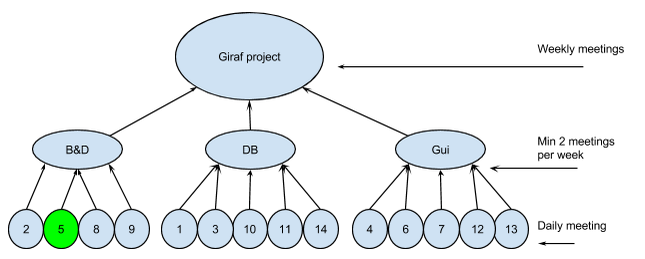
\includegraphics[width= 0.8 \textwidth]{pictures/ScrumOfScrum.png}
				\end{figure}
			\end{column}%
		\end{columns}
	\end{center}
\end{frame}

\begin{frame}
	\begin{center}
		\frametitle{Redmine}
		\begin{figure}[H]
			\centering
			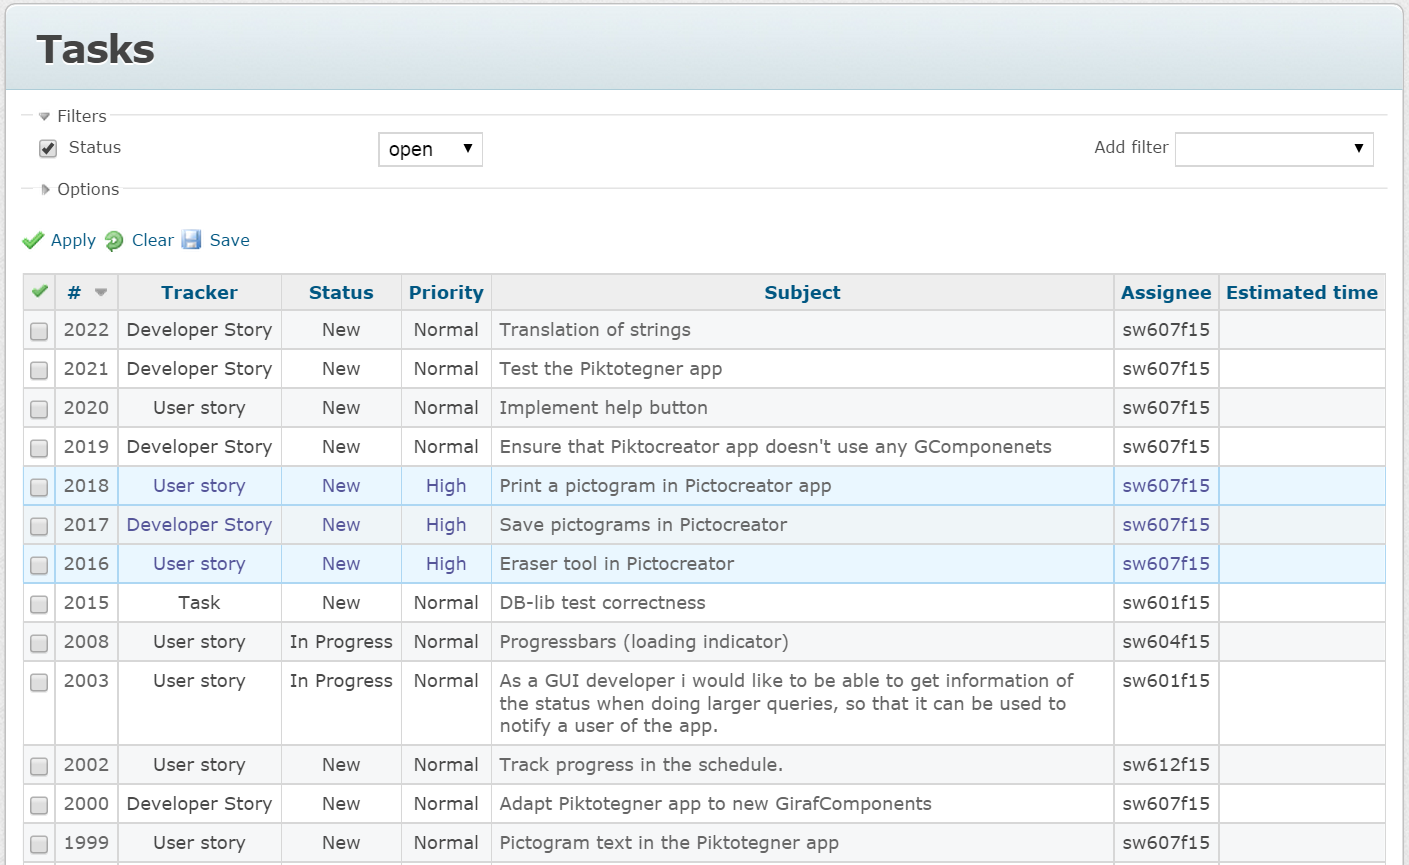
\includegraphics[width= 0.8 \textwidth]{pictures/RedmineStory.png}
		\end{figure}
	\end{center}
\end{frame}

\section{Product Owner}

\begin{frame}
	\begin{center}
		\frametitle{Responsibilities}
		\begin{columns}[T] % align columns
			\begin{column}{.48\textwidth}
				\begin{itemize}
					\item User stories
						\begin{itemize}
							\item Product Backlog
							\item Release Backlog
						\end{itemize}
					\item Sprint Planning
					\item Sprint End
					\item Communicate with other PO-groups
				\end{itemize}
			\end{column}%
			\hfill%
			\begin{column}{.48\textwidth}
				\begin{figure}[H]
					\centering
					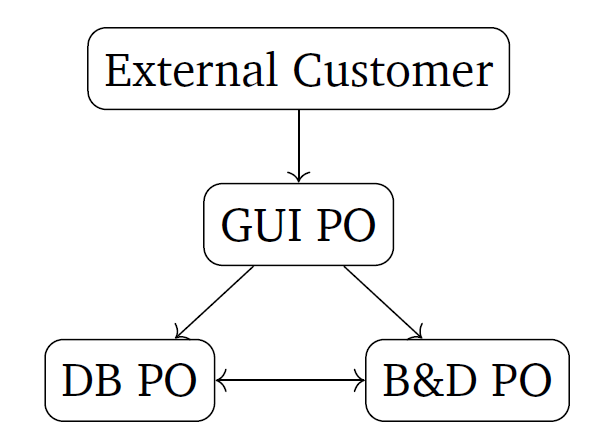
\includegraphics[width= 0.8 \textwidth]{pictures/ProductOwnerRelation.png}
				\end{figure}
			\end{column}%
		\end{columns}
	\end{center}
\end{frame}

\subsection{User stories}

\begin{frame}
	\begin{center}
		\frametitle{User stories}
	\end{center}
\end{frame}

\subsection{Backlog}

\begin{frame}
	\begin{center}
		\frametitle{Product Backlog}
	\end{center}
\end{frame}

\begin{frame}
	\begin{center}
		\frametitle{Release Backlog}
	\end{center}
\end{frame}
